\documentclass[12pt,a4paper]{article}
\usepackage[utf8]{inputenc}
\usepackage[english]{babel}
\usepackage{amsmath}
\usepackage{amsfonts}
\usepackage{amssymb}
\usepackage{graphicx}

\title{CAGD Exercise 3}
\author{Hanna Huber e0925230\\Stefan Zaufl e0925357}

\begin{document}
\maketitle
\section{Task 1}
The goal of this task was the computation of the interpolated spline of a set of points. We had a look at three methods for generating the knot vectors: equidistant, Chord and Lee. For the $C^1$-continuity we used FMILL and Bessel to estimate the first order derivation. \\
The different knot vectors are illustrated in Figure \ref{fig:knotvec}. The results for the corresponding algorithms can be seen in Figures \ref{fig:compC1Bessel} ($C^1$-continuous case) and \ref{fig:C2} ($C^2$-continuous case). There is not too much difference, but this might be the case because the points are nearly equidistant to their neighbors. \\
The $C^1$-continuous curves for different first derivative estimations can be compared in Figure \ref{fig:compC1Lee}. In our example, the FMILL method looks almost like a polygonal line. The Bessel method produces much rounder transitions, but the lack of $C^2$-continuity is clearly visible. This can be verified in Figure \ref{fig:C1vsC2}, where $C^1$-continuous and $C^2$-continuous spline interpolation are compared directly. 


\begin{figure}[hbtp]
\centering
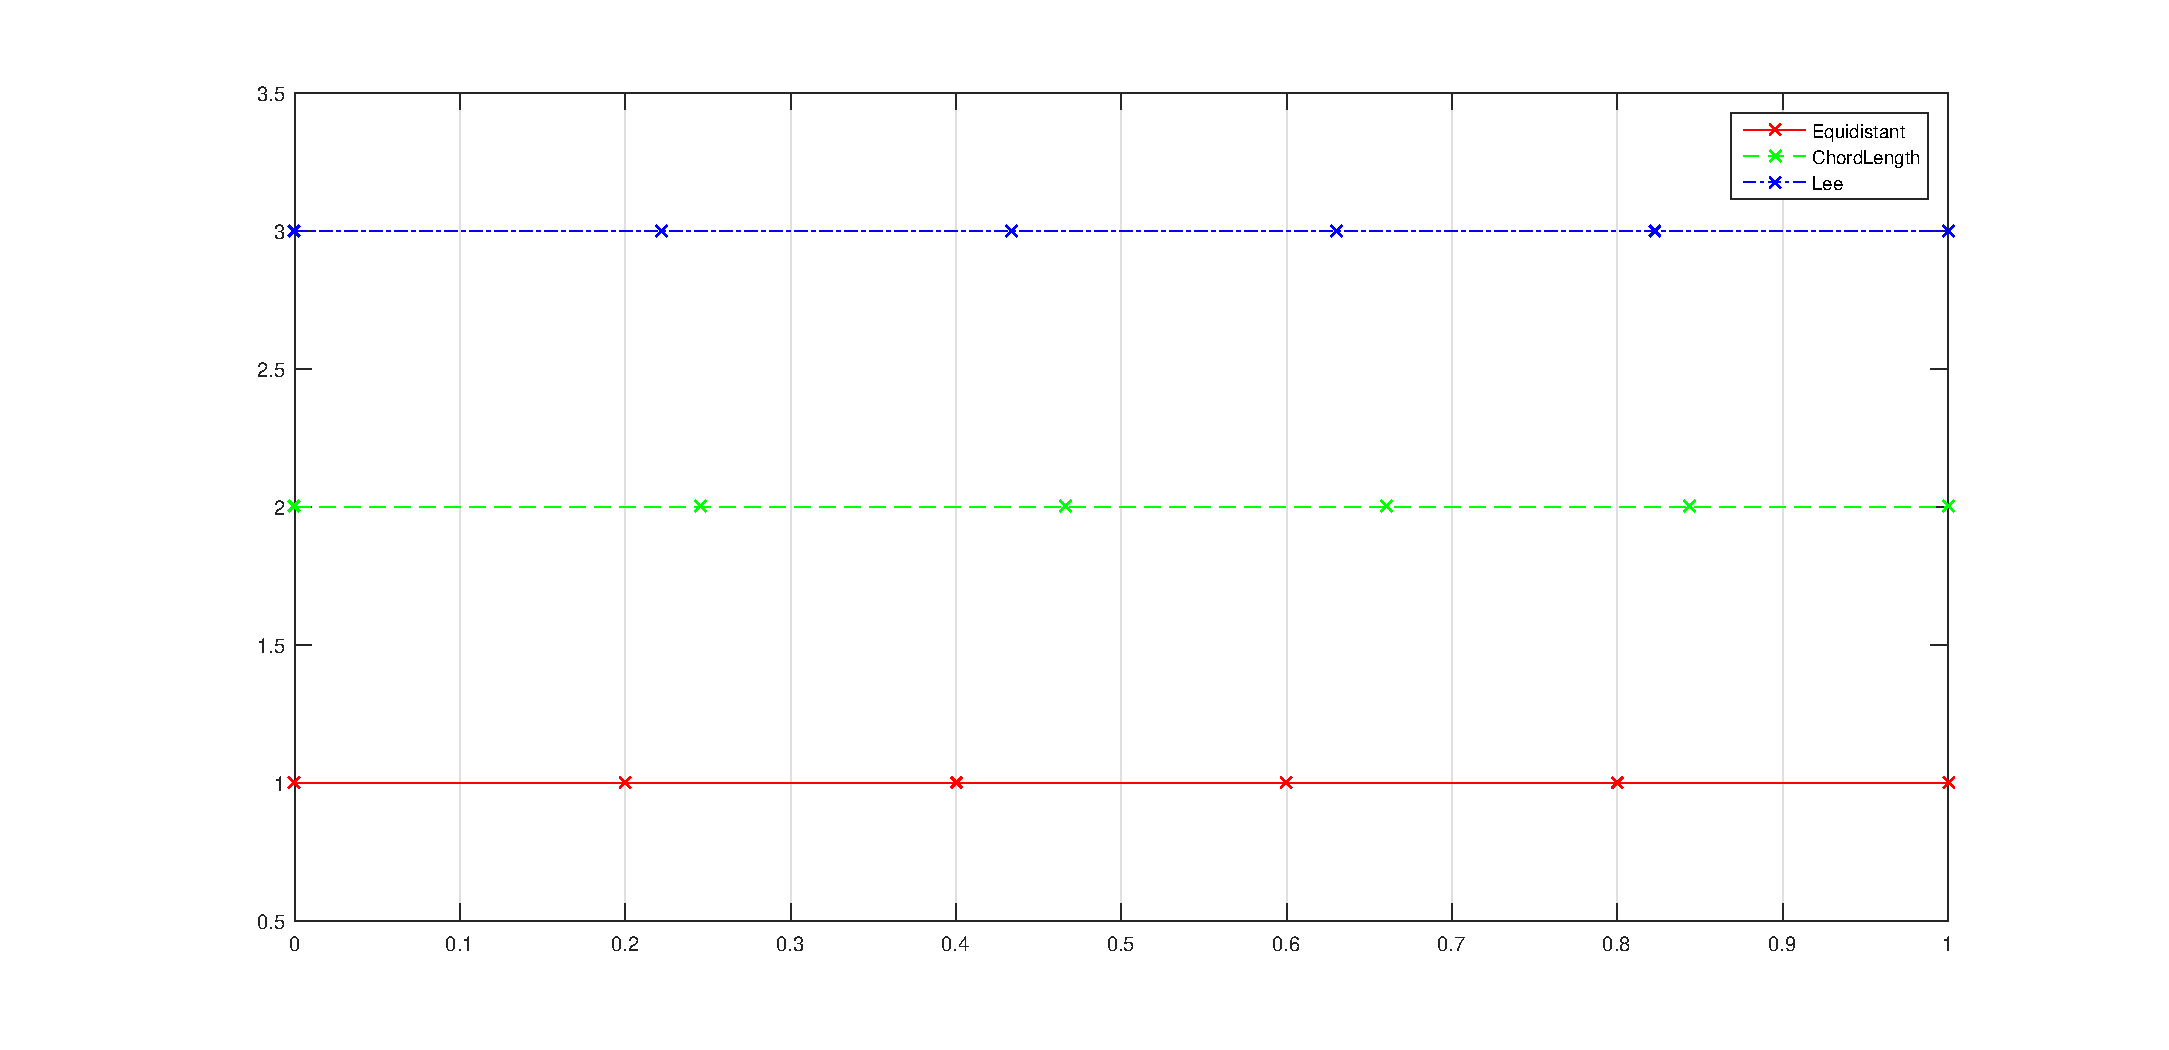
\includegraphics[width=\textwidth]{knotvectors.eps}
\caption{The different knot vectors yielded for our example curve.}
\label{fig:knotvec}
\end{figure}

\begin{figure}[hbtp]
\centering
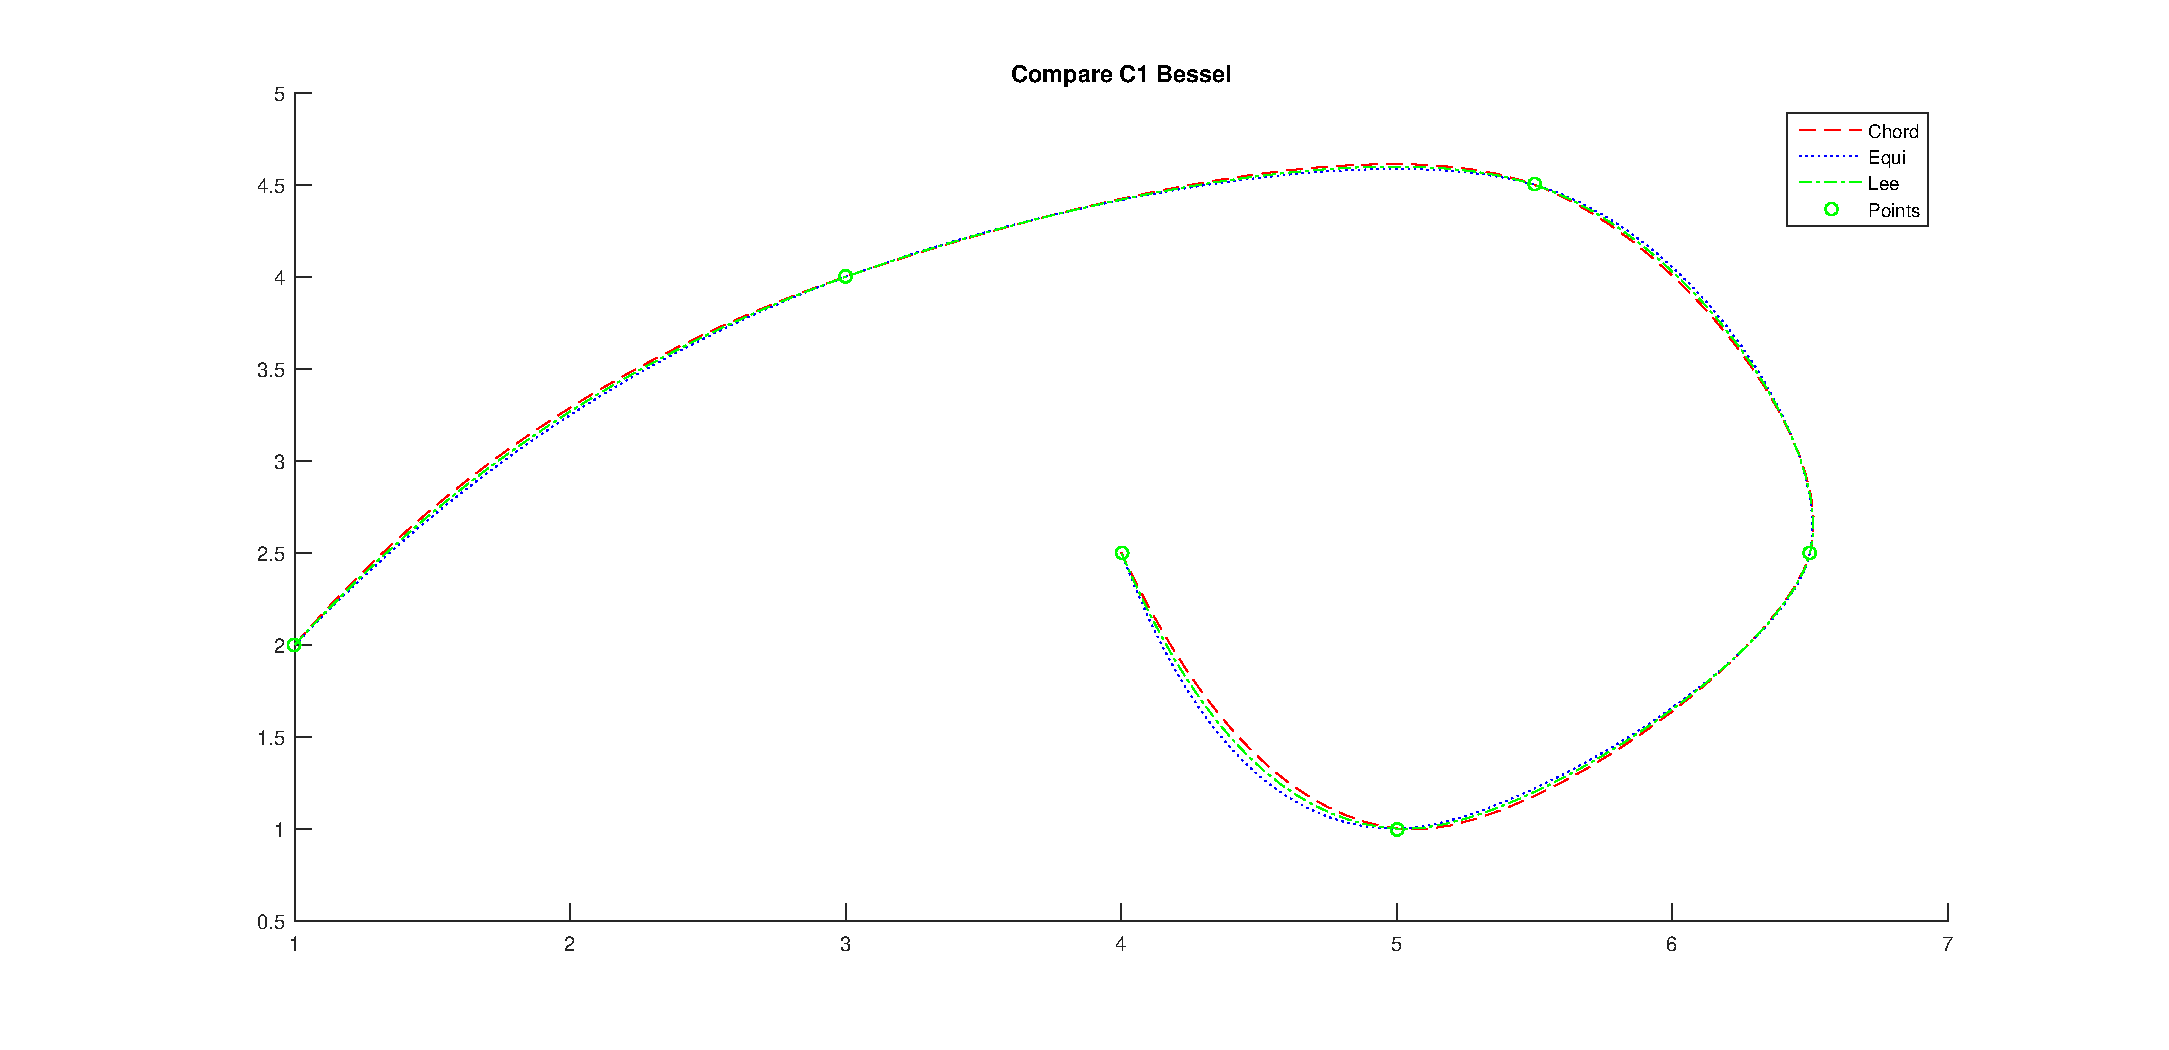
\includegraphics[width=\textwidth]{compC1Bessel.eps}
\caption{Comparison between the diffrent knot algorithms using the Bessel derivation estimation for a  $C^1$-continuity.}
\label{fig:compC1Bessel}
\end{figure}

\begin{figure}[hbtp]
\centering
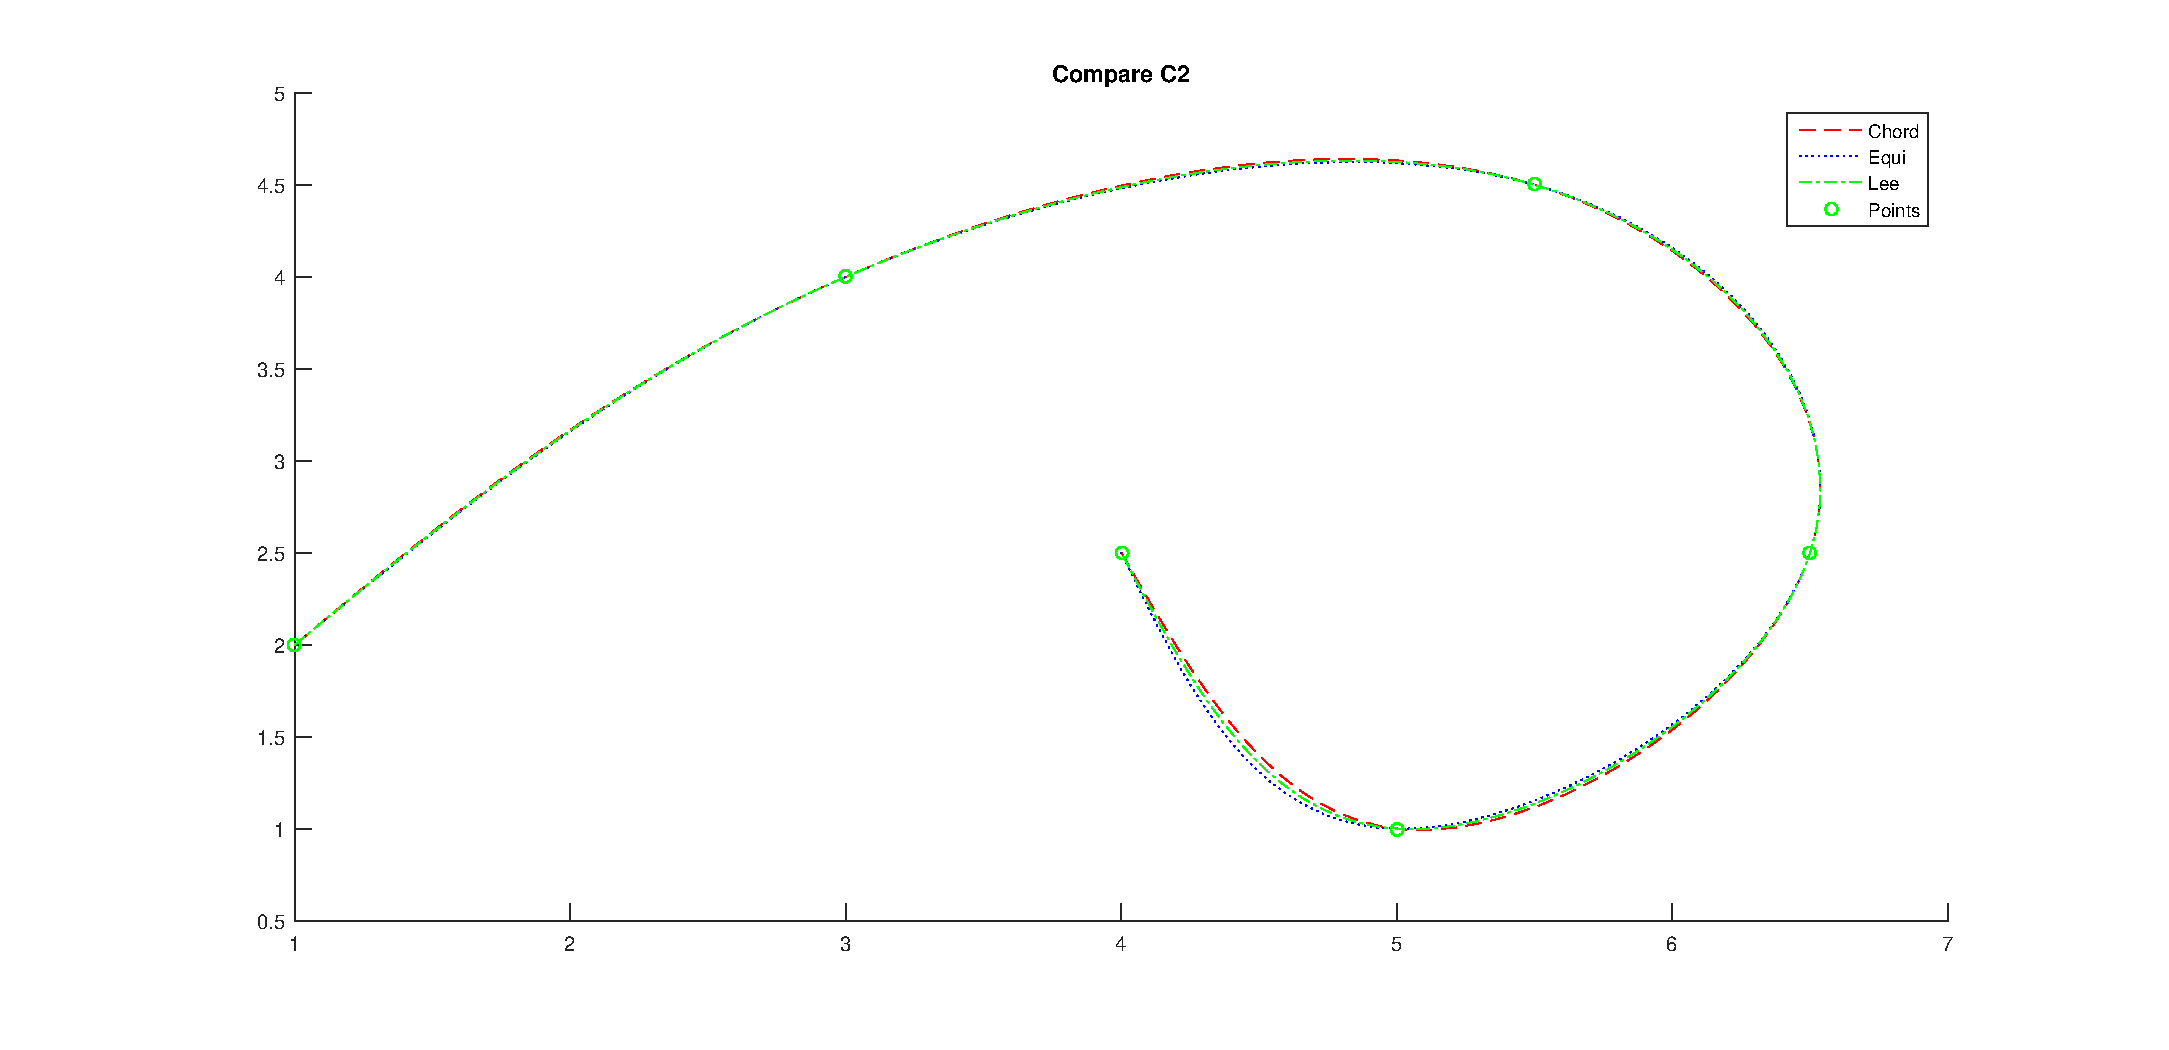
\includegraphics[width=\textwidth]{compC2.eps}
\caption{$C^2$-continuous interpolation for different knot vectors.}
\label{fig:C2}
\end{figure}

\begin{figure}[hbtp]
\centering
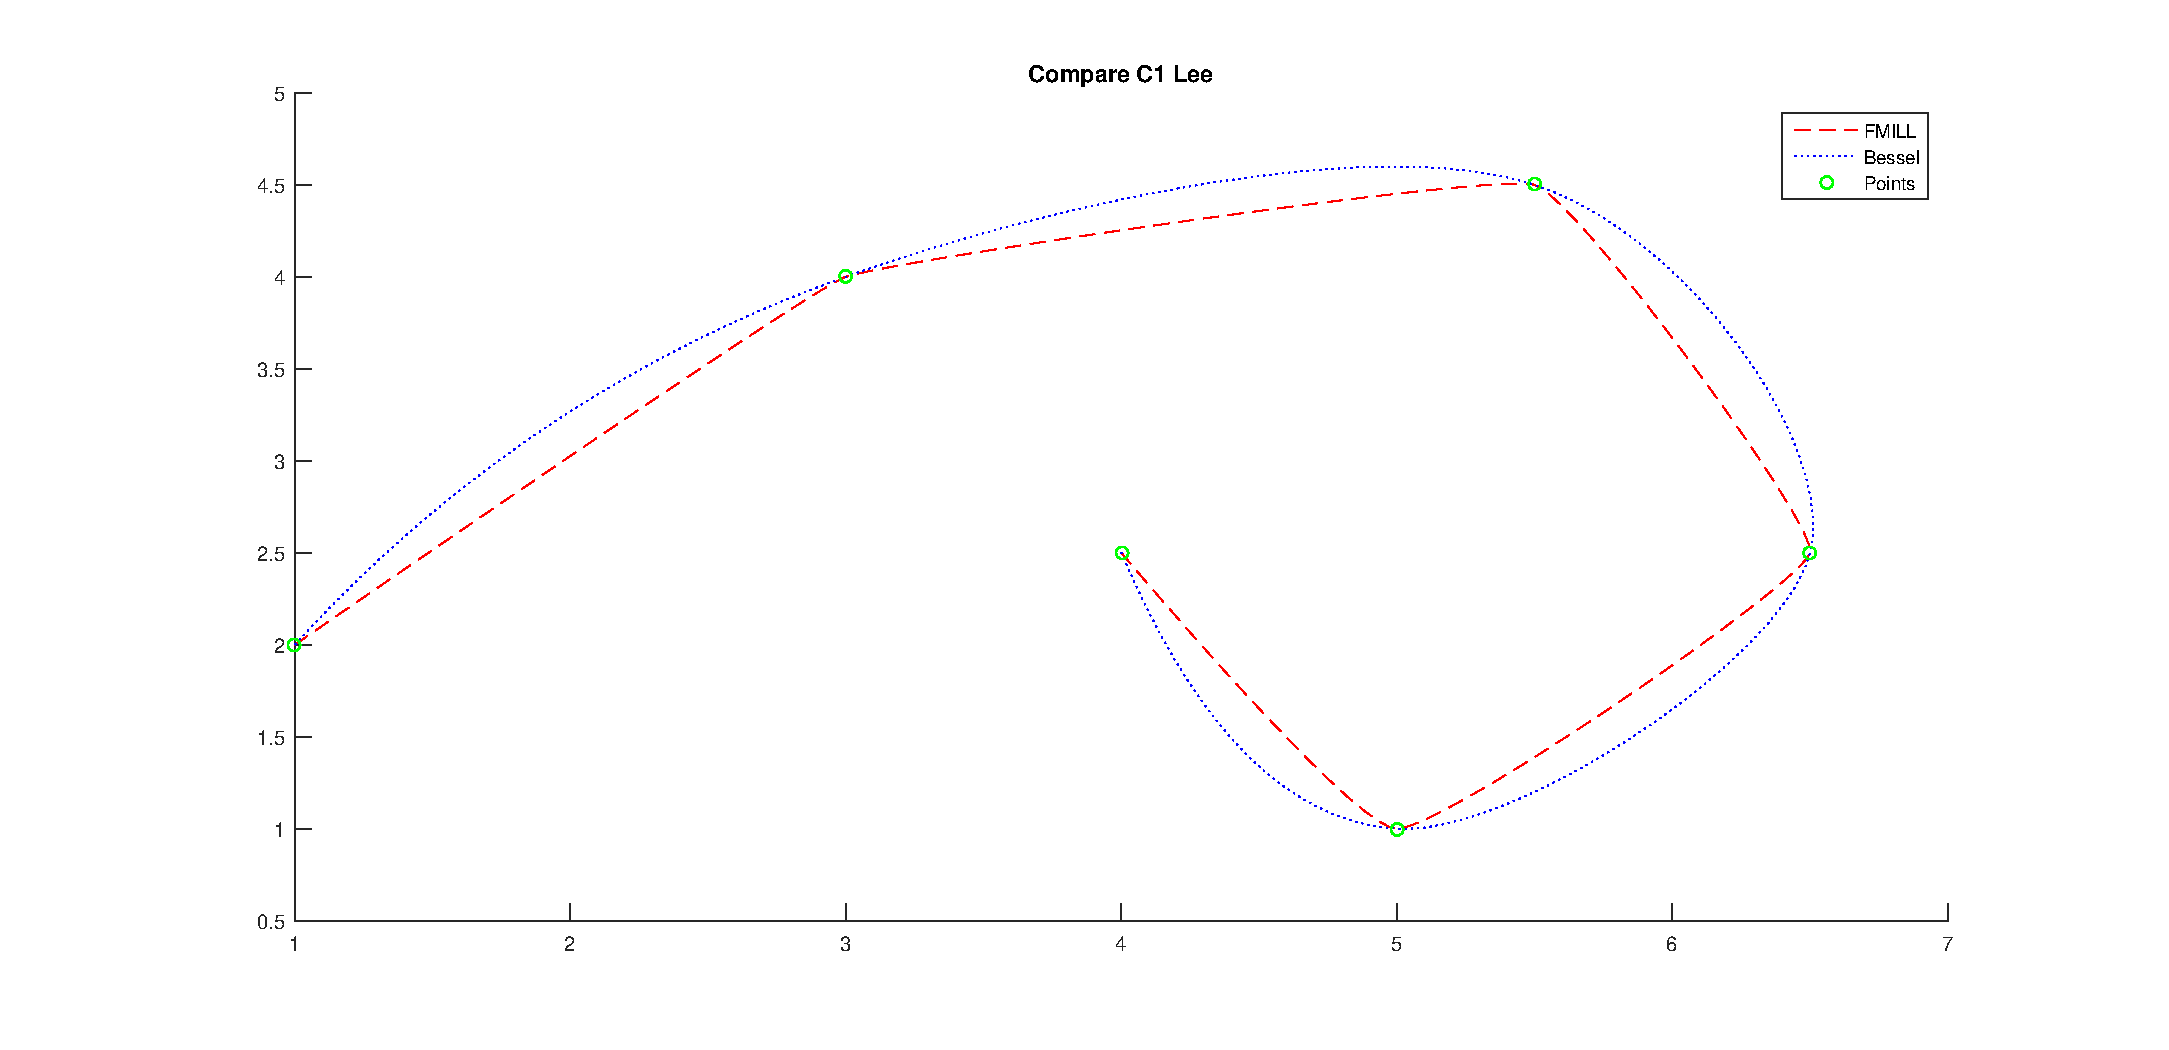
\includegraphics[width=\textwidth]{compC1Lee.eps} 
\caption{Comparison between the different derivation estimation methods for  $C^1$-continuity using the Lee knot algorithm.}
\label{fig:compC1Lee}
\end{figure}

\begin{figure}[hbtp]
\centering
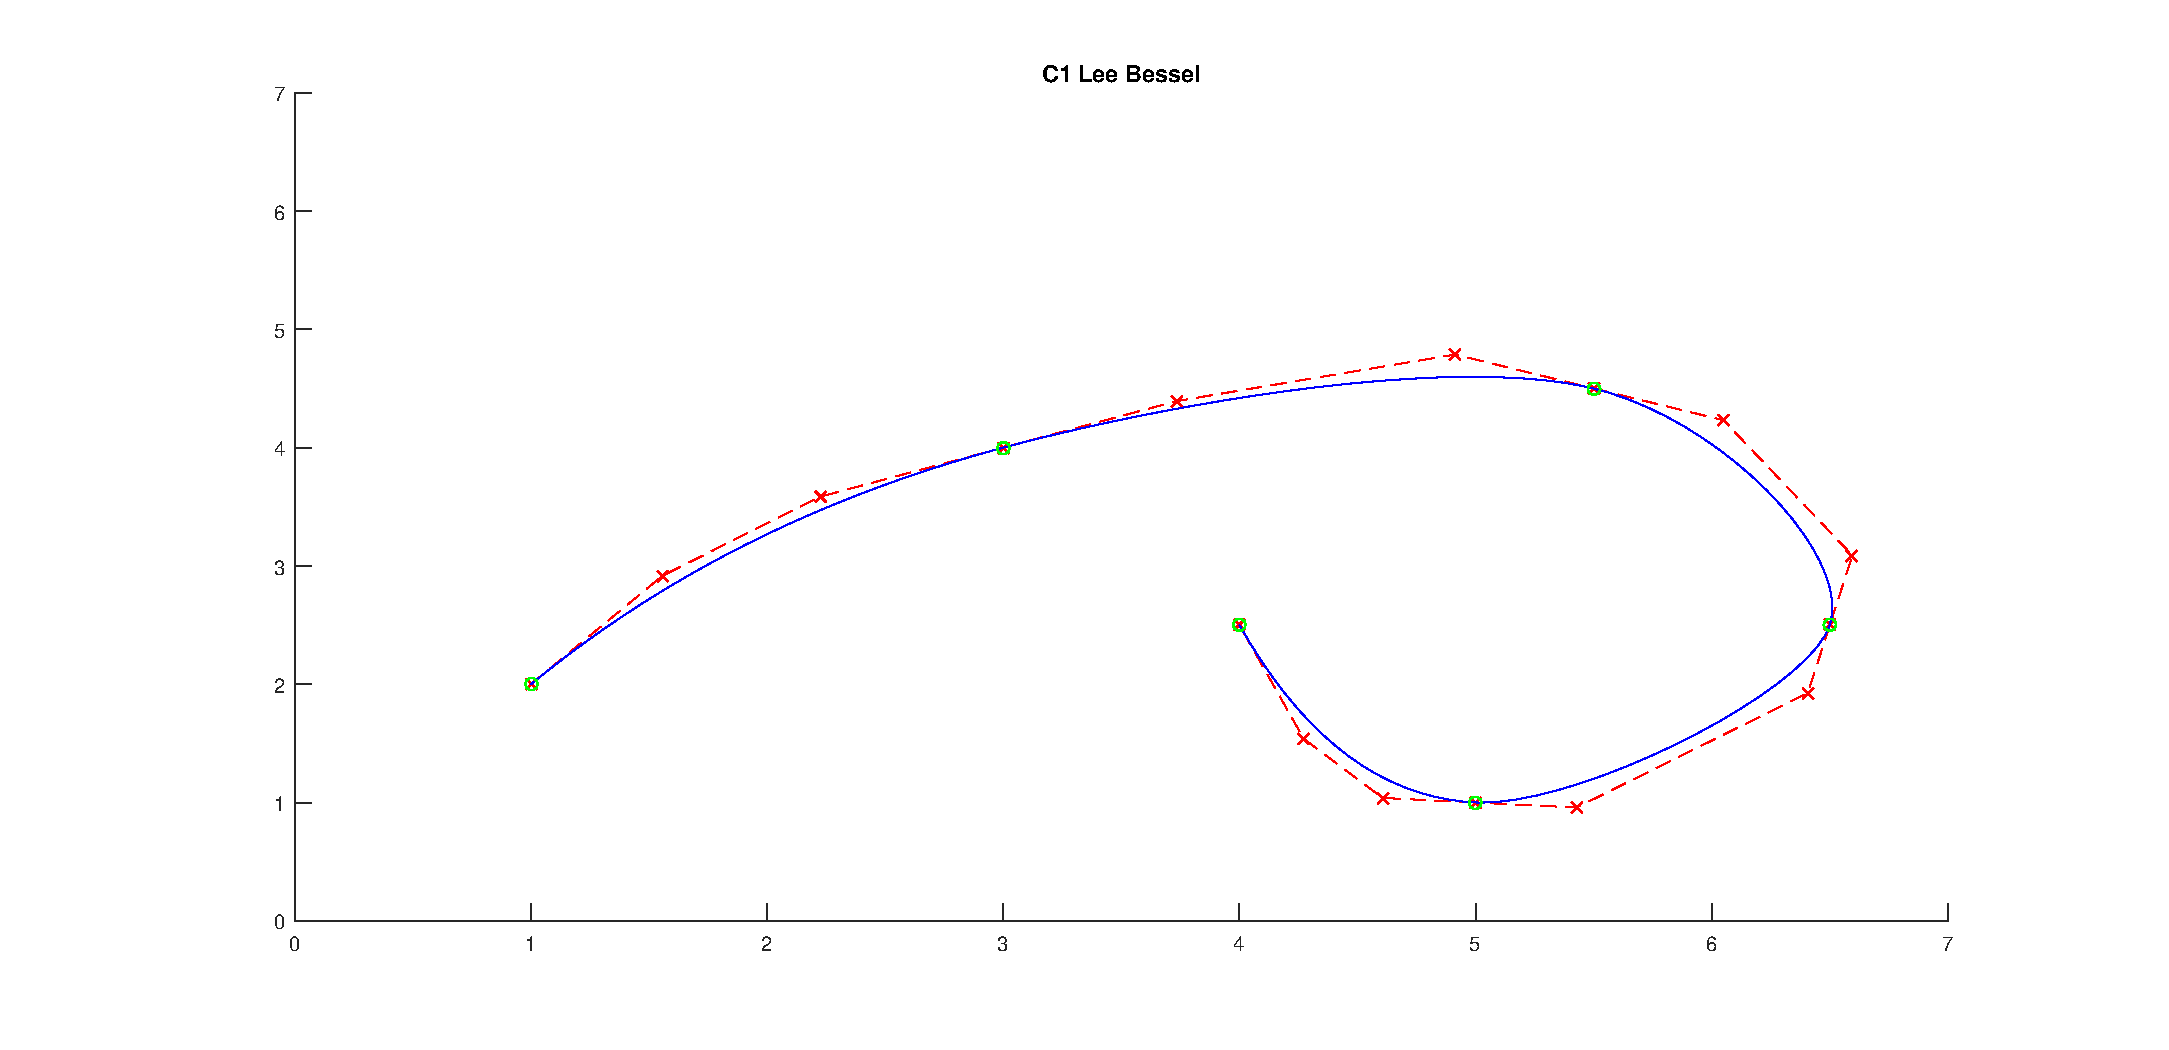
\includegraphics[width=\textwidth]{C1-LeeBessel.eps}
\caption{Showing the results of the Lee-Bessel method with the control polygons of the cubic curves.}
\label{fig:C1-LeeBessel}
\end{figure}



\begin{figure}[hbtp]
\centering
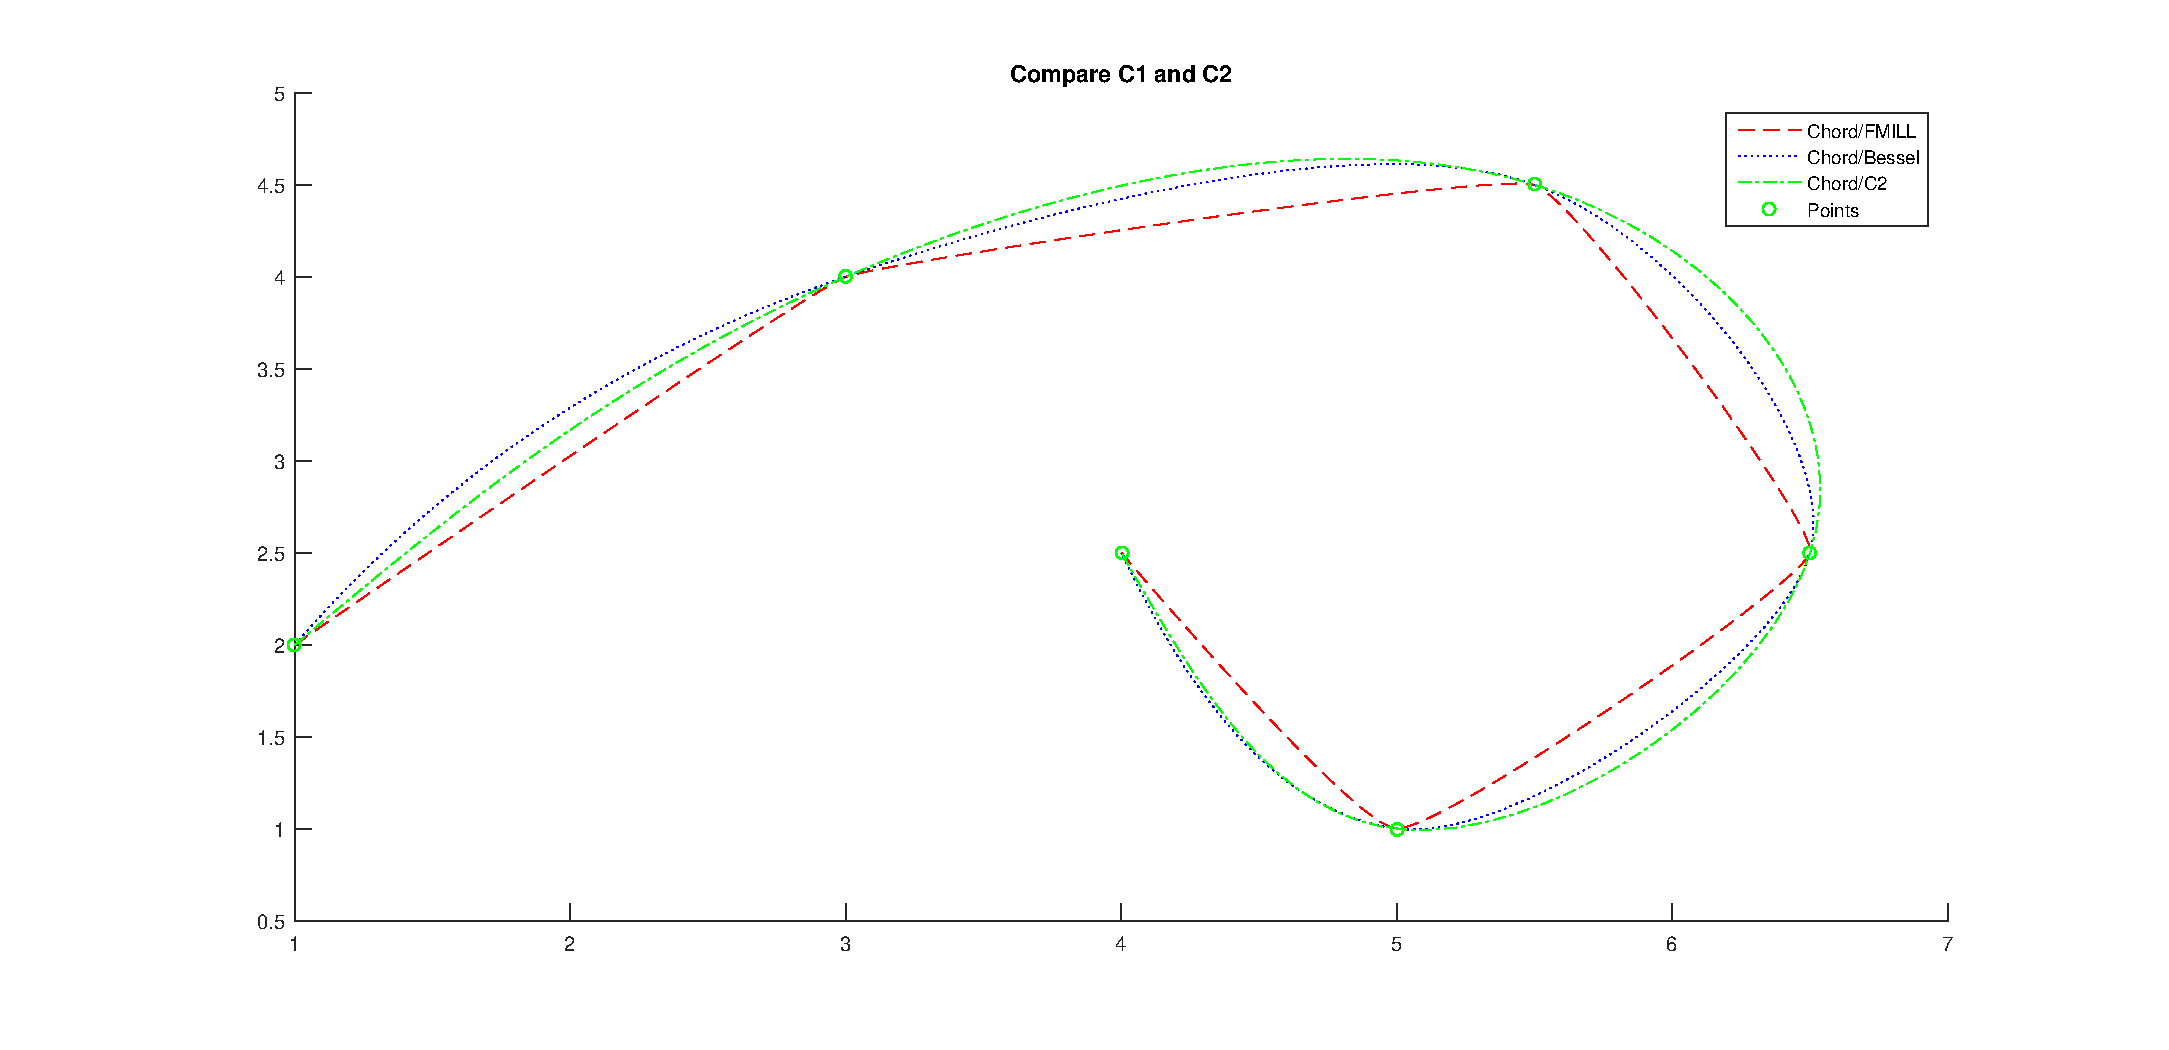
\includegraphics[width=\textwidth]{C1vsC2.eps}
\caption{Comparison  between  $C^1$-continuous spline interpolation with FMILL and Bessel-based derivatives and $C^2$-continuous interpolation.}
\label{fig:C1vsC2}
\end{figure}


\end{document}